% Created 2023-05-21 Sun 14:58
\documentclass[9pt, b5paper]{article}
\usepackage{xeCJK}
\usepackage[T1]{fontenc}
\usepackage{bera}
\usepackage[scaled]{beraserif}
\usepackage[scaled]{berasans}
\usepackage[scaled]{beramono}
\usepackage[cache=false]{minted}
\usepackage{xltxtra}
\usepackage{graphicx}
\usepackage{xcolor}
\usepackage{multirow}
\usepackage{multicol}
\usepackage{float}
\usepackage{textcomp}
\usepackage{algorithm}
\usepackage{algorithmic}
\usepackage{latexsym}
\usepackage{natbib}
\usepackage{geometry}
\geometry{left=1.2cm,right=1.2cm,top=1.5cm,bottom=1.2cm}
\usepackage[xetex,colorlinks=true,CJKbookmarks=true,linkcolor=blue,urlcolor=blue,menucolor=blue]{hyperref}
\newminted{common-lisp}{fontsize=\footnotesize} 
\author{deepwaterooo}
\date{\today}
\title{ET 框架拖拉机项目试改装}
\hypersetup{
  pdfkeywords={},
  pdfsubject={},
  pdfcreator={Emacs 28.2 (Org mode 8.2.7c)}}
\begin{document}

\maketitle
\tableofcontents


\section{双副牌双升108 张卡牌游戏}
\label{sec-1}
\begin{itemize}
\item 【游戏可试玩程序】:放在Release/Tractor.exe. Windows 用户大家可以下载试玩儿体验一下。
\item 昨天晚上找见了别人几年前就开发出来的卡五星麻将,所以写麻将游戏的想法就被恶杀在摇篮中。现在再写什么好呢?就只能写【双升拖拉机】了,就是两副牌108 张来打的拖拉机。现已经 ios iPhone 上有的双升游戏,可能搜索一下设计,写安卓版的双升了,看下能否套用ET 框架,写成四人网络【客户端与服务器双热更新的】网络游戏
\item 现在先搜索必要的框架设计,出版规则比大小算法之类的。
\item 【服务器与客户端的同步】:尤其是在分四人牌后,亮主拖底的时候,谁先亮,亮什么主,顺序重要,结果重要。【 ET 框架有专用的游戏服,由游戏服来状态同步】在本程序中,采用的是服务器保存所有的状态,处理所有的逻辑。比如,客户端在点击亮主后,做的事情就是发一个消息给服务器,不做任何显示操作,等待服务器传来亮主的消息后再显示
\begin{itemize}
\item 【发牌,公正性】:随机分牌。第一步就是要发牌。需要做到一个完全随机的发牌,就要保证每张牌发到每个玩家手里的概率都是一样的,而且牌的顺序是等概率随机打乱的。程序中采用的是如下的发牌算法(感谢Dr.Light提供):假如有两幅牌,编号从1到108,首先随机选出一个,并且将牌发给玩家,然后将这个编号的牌与108号牌交换编号,那么剩下的牌就是从1到107号。于是再从中选出一个,重复以上的过程,这样一来,算法的复杂度就是O(n)。
\end{itemize}
\end{itemize}
\section{主要想要改进的地方:前辈十年前开发出的游戏,游戏整体【差强人意】现官宣的现项目基础上,主要游戏逻辑与改进方向【除了重构适配ET 框架以实现客户端服务器双端热更新, besides之外】如下。}
\label{sec-2}
\begin{itemize}
\item \textbf{【界面设计:】} 八十年前没有ET 框架,不知道原作者是如何设计这个游戏的。感觉游戏的整体走桌面游戏风,要把菜单设计等改成【手游风格】。
\item \textbf{【逻辑设计,用户意愿:】} 不【尊重用户游戏配置选择】的游戏,永远是固执不受欢迎的。【游戏逻辑、玩法】需要能够给用户留足选择配置空间,如下:
\begin{itemize}
\item 现有的游戏规则:再找了理解一下:现找到原项目中提到这些。但作为程序员,不把它所有相关逻辑读懂,都感觉不明白它说的狠多是什么意思
\end{itemize}
\end{itemize}

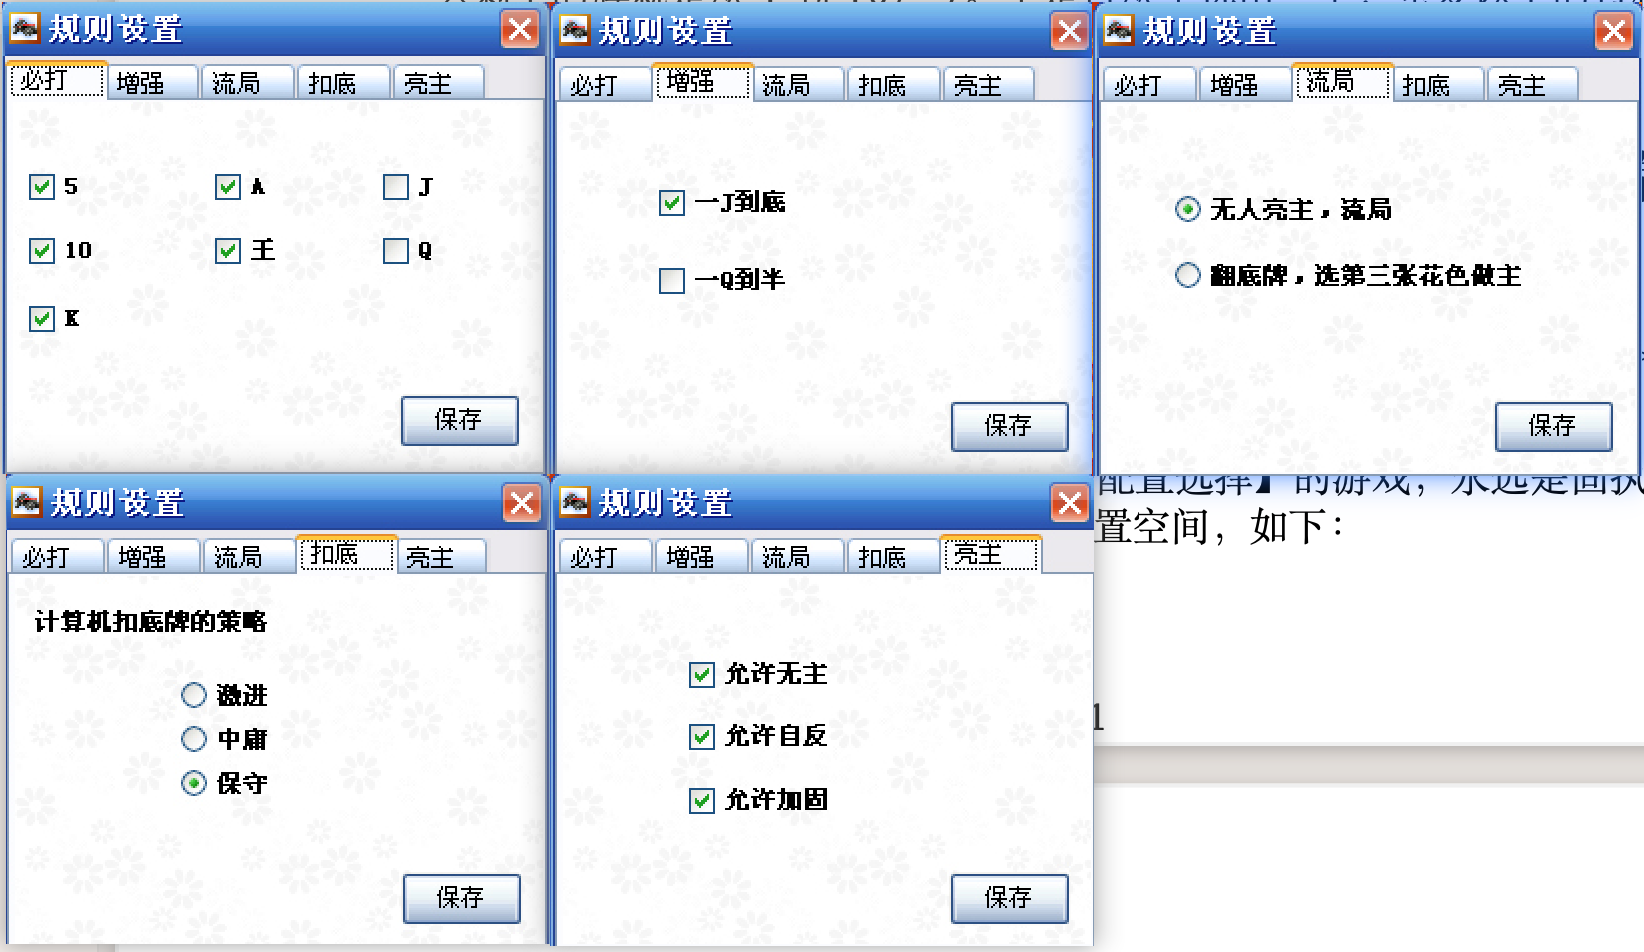
\includegraphics[width=.9\linewidth]{./pic/readme_20230510_160604.png}

\begin{center}
\begin{tabular}{ll}
\textbf{2 为常主} & 是常主,就常主会比较多,否则常主少,尤其打王的时候\\
\textbf{5 10 K 必打} & 因为比较难打\\
\textbf{单 J 勾到6, 双 JJ 勾到 2} & 开历史倒车,增加游戏的无穷乐趣:惊险刺激:逢对家对J, 谁不想把对方废到6 或是2?\\
 & 逢自家打到J, 会想要被对方废到6 或是2?\\
\textbf{逢 J 必打} & 因为上面不能言说的【惊险刺激】,不给任何双方逃跑的好玩机会\\
\textbf{小光升1 级,大光连升3 级} & 不满 40 算小光,0 分为大光头。。。连升三级\\
\textbf{捡分方扣底,底分翻倍} & 单扣乘2, 又扣乘 4, 拖拉机扣牌数乘 2.\\
 & 如此,才能让捡分方快速超越,以风马牛不能及之势火箭升级。。。\\
\end{tabular}
\end{center}
\begin{itemize}
\item \textbf{【关于J Q】}, 游戏设置: 
\begin{itemize}
\item 增强的规则:在一些地方流行一J到底、Q到半的玩法。
\item 庄家在打J时,如果下台,并且最后一把被J抠底,那么此庄家再上台时将从2开始打。
\item 庄家在打Q时,如果下台,并且最后一把被Q抠底,那么此庄家再上台时将从6开始打。
\end{itemize}
\item \textbf{【亮主规则】} :可以选择是否允许自反,加固和亮无主
\item \textbf{【亮牌规则】} :(注:以打8为例) \textbf{【这里有狠大的游戏逻辑改进,和游戏用户体验提升空间】}
\begin{itemize}
\item 在发牌过程中,第一次亮出的8的花色作为主牌花色。
\item 有以下几种情况可改变或加强主牌花色:
\begin{itemize}
\item 自保
\item 反主
\end{itemize}
\item 以上后三条以先出现者为准。
\item 若发牌结束仍无人亮牌,则以底牌第一张的花色作为主牌花色。
\end{itemize}
\item 以上三点应该是自己着重想要改进的地方
\item \textbf{【流局规则】} :如果摸牌时无人亮主,那么有两种选择,一是【流局】,重新发牌,二是【揭底】,将八张底全部揭开,选第三张牌的花色作为主花色。感觉流局设置不太好玩,浪费时间。
\item \textbf{【扣底规则】} :计算机在扣牌时,有三种扣牌算法可供选择:这里说的应该是,机器人应对其它三个玩家时的扣底规则,放8 张底牌,如何放原则。
\begin{itemize}
\item 1.激进算法,以扣绝一门为主要目标
\item 2.中庸算法,以不扣分(5分除外)为主要目标
\item 3.保守算法,以不扣分不扣对为主要目标
\end{itemize}
\item \textbf{【升级规则】}
\begin{itemize}
\item 闲家得0分为大光,庄家升三级。
\item 闲家得分小于40分为小光,庄家升二级。
\item 闲家得分大于等于40分且小于80分时,庄家升一级。
\item 闲家得分大于等于80分且小于120分时,闲家上台。
\item 闲家得分大于等于120分且小于160分时,闲家上台且升一级。
\item 闲家得分大于等于160分且小于200分时,闲家上台且升二级。
\item 闲家得分大于等于200分时,闲家上台且升三级。
\end{itemize}
\item \textbf{【打牌规则】} :(注:以打10为例) \textbf{出牌时同等大小的牌以先出者为大。}
\begin{itemize}
\item \textbf{同门花色的大牌可以联出,称作“甩牌”} 如:
\item 副牌中:AAK,AKK,AQQJJ,
\item 98844(若其他家中无人有能大过一张9,和一对8,和一对4的牌)。
\item \textbf{若首家试图联出的牌并非都是大牌时,则其必须出欲联出的牌中的最小牌。} 如:
\begin{itemize}
\item 首家试图联出98844时,若其余某家有此花色的J,则首家必须出9,若其余某家有此花色的QQ或55,则首家必须出44。
\item 首家出对牌时,其余家有对牌必须出对牌(包括拖拉机中的对牌)
\item 首家出拖拉机时,其余家有拖拉机必须出拖拉机,若无拖拉机,则必须出对牌,无对牌时才能出其它牌。
\end{itemize}
\item \textbf{首家出某花色副牌时,其余家无此门花色时,可出主牌,称为“毙”。} 若首家出的牌中有拖拉机或对牌,毙牌时所出的牌必须是主牌,且其拖拉机的数目不得少于首家出的牌中的拖拉机的数目,对牌的数目也不得少于首家出的牌中的对牌的数目,否则被视为垫牌。
\item *出现多家毙牌时,毙牌的大小以毙牌中的拖拉机和对牌大小为准,大的称为“盖毙”。*如:
\begin{itemize}
\item 主牌998872可毙副牌AK5544,但不能毙副牌AA5544
\item 主牌977可毙副牌544,主牌884可盖毙
\item 主牌977可毙副牌567,主牌884不能盖毙
\end{itemize}
\end{itemize}
\item \textbf{【抠底规则】} :
\begin{itemize}
\item 以单张牌抠底时底牌分数乘二。
\item 以对牌牌抠底时底牌分数乘四。
\item 以拖拉机抠底时底牌分数乘八 \textbf{【应该是拖拉机张数乘以2】} 。因为大拖拉机可以三对四对。。。或留底甩牌,只要能大。。。
\end{itemize}
\item \textbf{【拖拉机的构成】} :(注:以打10为例)
\begin{itemize}
\item \textbf{凡大小顺序相邻且花色相同的联对均构成拖拉机} ,如:
\begin{itemize}
\item KKQQ,JJ99,554433;
\end{itemize}
\item \textbf{主牌中凡大小顺序相邻联对均构成拖拉机} ,如:
\begin{itemize}
\item 一对小王带一对主10,一对主10带一对副10
\item 一对副10带一对主牌A,一对主10带一对副10及一对主牌A
\end{itemize}
\item 以下各例均不是拖拉机:
\begin{itemize}
\item 554,544,5533,JJQQ,两对副10,JJ1010,AA22
\end{itemize}
\end{itemize}
\item \textbf{【牌的大小顺序】} :现在游戏框架设计,束缚了用户的 \textbf{【2 为常主】} 的 \textbf{配置选择,算法,数据结构等,需要重构}
\begin{itemize}
\item 以打10为例
\item 主牌从大至小依次为:
\begin{itemize}
\item 大王,小王,主10,副10,A,K,Q,J,9,8,7,6,5,4,3,2
\end{itemize}
\item 副牌从大至小依次为:
\begin{itemize}
\item A,K,Q,J,9,8,7,6,5,4,3,2
\end{itemize}
\end{itemize}
\item \textbf{【轮庄规则】} :为创造出好玩儿的玩法,这里是可以优化改进的。对家的本意是,两人合作,快速升级,所以需要两者配合。不需要,或可以配置不规定严格的顺序,给予他们无数无限合作可能,给予对方继续反副反主的机会,增加游戏趣味。
\begin{itemize}
\item 开局中,双方争庄,先亮者为庄家。
\item 庄家升级时,下一副牌由其对家当庄家。
\item 闲家上台时,下一副牌由此副牌的庄家的下家当庄家。
\end{itemize}
\item 其它这里没有列出来的,主要是我现在还不曾了解那些是在说什么,比如下面网络上提到过的:提供六种配置选项: \textbf{【允许自反】,允许对家保,允许反无将,A 必打} (是为什么呢,K 易跑光,不好捡分?)等
\item \textbf{【点击触屏、用户交互的性能优化】} :需要优化。玩家就算玩得不久,一直点鼠标,也是痛苦的事。需要AI 辅助,智能帮助用户出牌,让鼠标点击、选牌聪敏、反应快。
\begin{itemize}
\item 原游戏应该是桌面游戏,所以会有快捷键设置。但手游,就需要自己将触屏设置优化出来
\end{itemize}
\item \textbf{【逻辑设计,用户意愿:】}: 逻辑上,为能实现以上种种好玩玩法,游戏逻辑需要 \textbf{规定,约束严格的反牌规则:从高到低为【王黑红梅方】} ,就是别人叫方块的主,其它都可以反,但若是已经反到黑桃,接下来就只能反王或说是常主。允许捡分方按照以上规则反牌,这样才给给予捡分方底牌放 80 分,拖拉机扣底,火箭升级的机会。规则明确,公正。现游戏中一个【“流局”】界面,抹杀了这一切好玩儿的过程与结果,太不好玩了。。。游戏界面,也需要必要的文字提示等,帮助玩家理解游戏中的这些好玩儿规则,让玩家上瘾。。。
\end{itemize}
\section{游戏整体【差强人意】现游戏试玩中抓到的【BUG:】如下}
\label{sec-3}
\begin{itemize}
\item 不考虑现代大型网络游戏的双端热更新机制。现在游戏的热更新实在是必备。游戏整体,逻辑相对完整,提供了完整的AI 辅助,主要只是提供了 \textbf{牌面的背景图、游戏桌面背景图、背景音效等配置} 。但 \textbf{游戏逻辑单一固定,不好玩。}
\begin{itemize}
\item 现有的游戏中已经配置如下:只有算法,以及游戏性能需要优化
\end{itemize}
\end{itemize}
\subsection{游戏}
\label{sec-3-1}
\begin{itemize}
\item \textbf{【开始新游戏】} :开始新的游戏,从2打起
\item \textbf{【暂停游戏】} :可以暂停游戏,再点击此菜单将继续游戏
\item \textbf{【保存牌局】} :将游戏的状态保存起来,包括各家在打几,庄家是谁,目前打几
\item \textbf{【读取牌局】} :读取保存的牌局,重新发牌
\end{itemize}
\subsection{设置}
\label{sec-3-2}
\begin{itemize}
\item \textbf{【游戏速度】} :可以设置游戏的每个步骤的速度,左边为快速,右边为慢速
\item \textbf{【牌面图案】} :有三种图案可供选择,你也可以选择自己制作的牌面
\item \textbf{【牌背图案】} :有三种背面图可供选择
\item \textbf{【牌桌图案】} :可以选择背景图案,图片大小为固定大小,如果不是这个尺寸,图片将进行缩放
\item \textbf{【背景音乐】} :可以设置打牌时的背景音乐,支持wav、mp3、midi三种音乐格式,可随机、循环播放
\item \textbf{【游戏规则】} :可以设置必打、增强(一J到底、一Q到半)、揭底、扣底、亮主等规则。 \textbf{【缺点:】} 对新玩家来说,这些概念不明确,需要游戏界面提醒
\item \textbf{【机器人罗伯特】} :这个机器人可以代替您打牌。 \textbf{【想把这个更多的用在,手游辅助触屏点击时】}
\end{itemize}
\subsection{工具}
\label{sec-3-3}
\begin{itemize}
\item \textbf{【拖拉机伴侣】} :使用这个工具可以制作您自己的牌面,将您的数码照片嵌入到游戏中【这个可能有点儿多余】。但仍可以手游上试执行。
\end{itemize}
\section{主要【BUG:】}
\label{sec-4}
\begin{itemize}
\item 对游戏整体的玩家用户体验如此,但并不是说我就真的狠懂这个游戏项目。实际上,我还没能真正学习这个项目,甚至它底层的算法动态库的连接等,都是我需要从这个十年前的项目中学习的地方。借他山之石,为自己的游戏所用。
\item 现在抓到的主要 bug 如下截图:
\end{itemize}

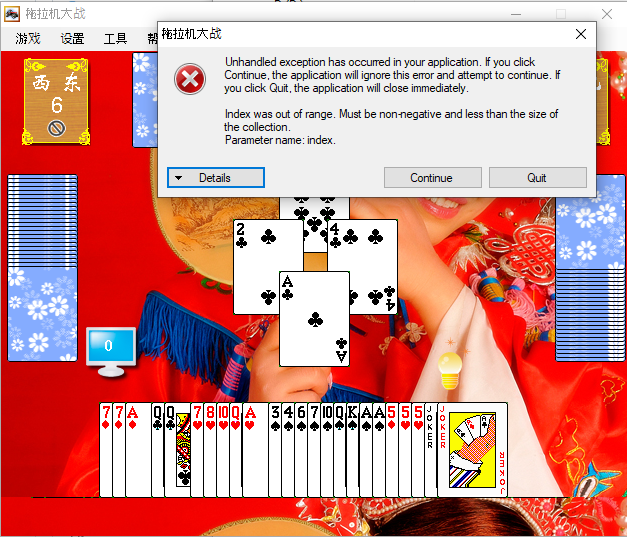
\includegraphics[width=.9\linewidth]{./pic/readme_20230509_230111.png}

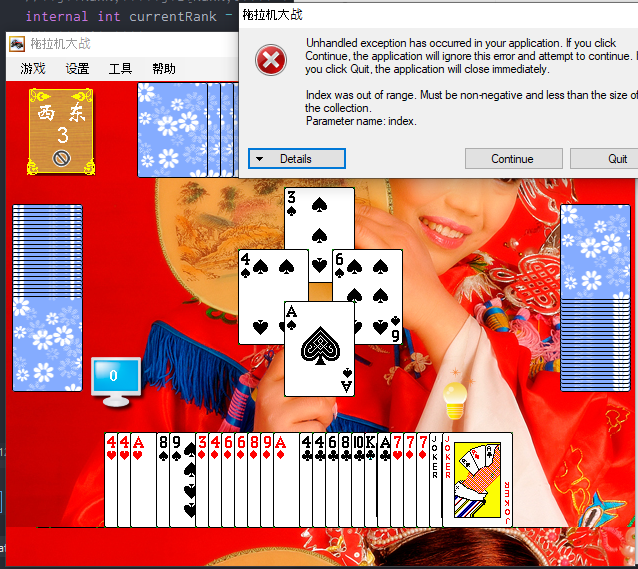
\includegraphics[width=.9\linewidth]{./pic/readme_20230509_232252.png}

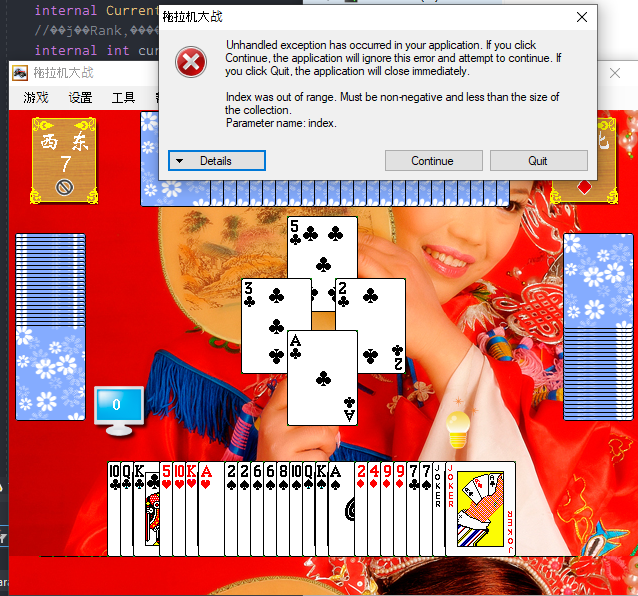
\includegraphics[width=.9\linewidth]{./pic/readme_20230510_014418.png}

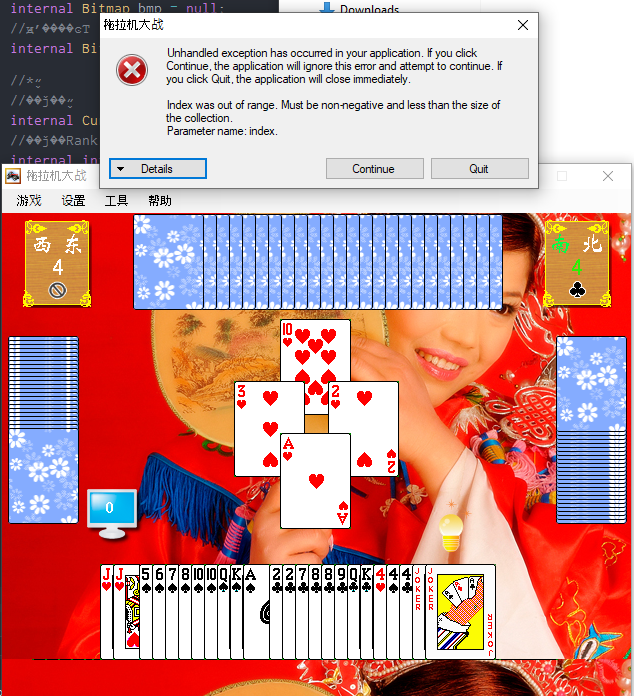
\includegraphics[width=.9\linewidth]{./pic/readme_20230510_015324.png}

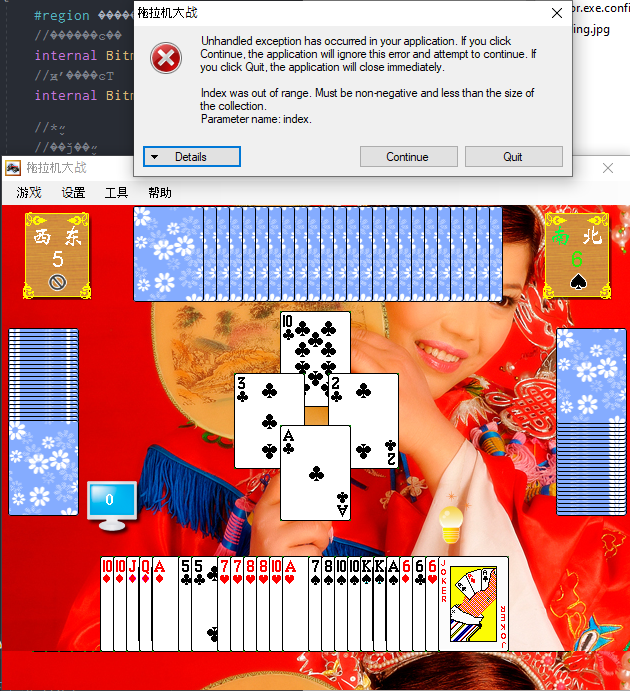
\includegraphics[width=.9\linewidth]{./pic/readme_20230510_033444.png}

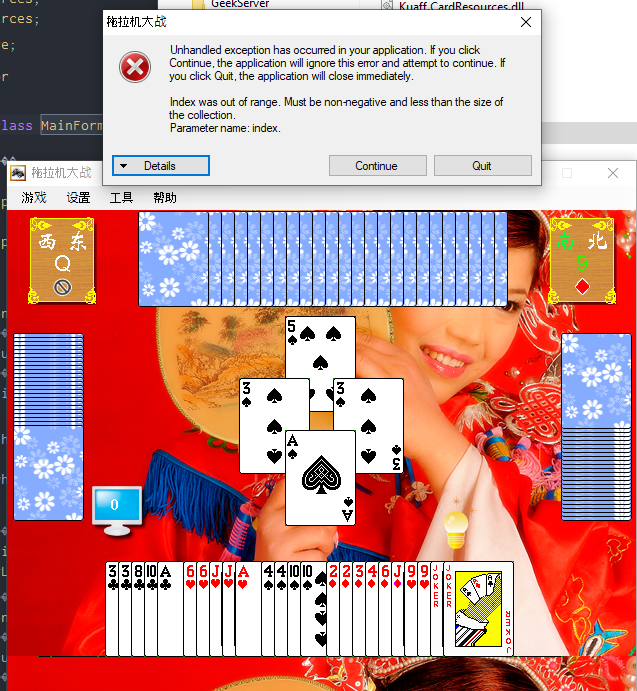
\includegraphics[width=.9\linewidth]{./pic/readme_20230510_042818.png}

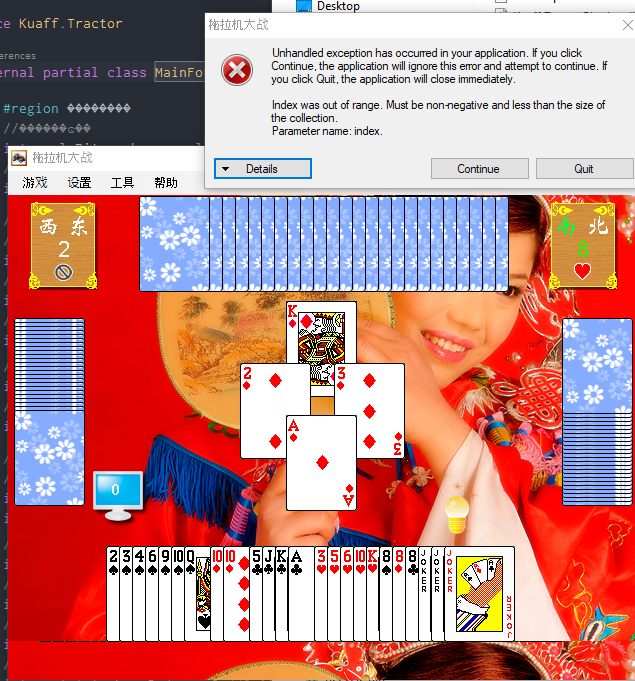
\includegraphics[width=.9\linewidth]{./pic/readme_20230510_043722.png}

\begin{itemize}
\item 【牌的逻辑OOD/OOP】设计:三个类,对应单张,拖拉机(对子是长度为1 的拖拉机),和混合单张与拖拉机
\item 简易版设计原理:模拟拖拉机(升级)玩法;
\begin{itemize}
\item 1.创建两副牌的集合:HashMap
\item 2.创建纸牌:四个花色共108张♦ ♣ ♥ ♠
\item 3.创建poker的ArrayList操作集合
\item 4.创建亮主牌的操作
\item 5.将所有牌放入牌盒中
\item 6.创建四个玩家与底牌的集合:HashSet wj1,wj2,wj3,wj4,dipai
\item 7.洗牌
\item 8.发牌操作
\item 9.创建看牌方法
\item 10.调用方法看牌
\end{itemize}
\item 安桌上的游戏现在是这样的:还要再写一个吗?【活宝妹就是一定要嫁给亲爱的表哥!!!】还是说更为完善或是好玩儿的游戏逻辑?或是UI 视图画面,或是性能表现?反正一定是套用ET 框架写得最容易快速方便。【感觉现在这个截图的UI 长得有点儿丑怪。。】不好看不经典,看了就不想玩儿了。。
\item 因为各处的游戏规则不一样,所以给玩家多点儿自由,自己选择玩法。提供六种配置选项:【允许自反】,允许对家保,2 为常主,允许反无将,五十K 必打,JA 必打等
\end{itemize}
\section{项目理解消化与游戏逻辑性能的进一步改装}
\label{sec-5}
\begin{itemize}
\item 重写这个经典游戏:两大主要目标:【套用ET 框架,实现客户端与服务器的热更新】主要是为深入理解一个大型网络服务器游戏热更新框架的练手;第二目标,把这个单机贺岁版的游戏弄得更好玩儿一点儿。
\item 如果想要修改主要亮牌过程与逻辑,就需要所有的玩家都各具备一个可以亮牌的框。帮助玩家提高游戏技能精准打牌,就是帮助游戏记忆。当玩家没能记住前一轮对家是否还有某门副牌的时候,可以提醒玩家。【黑红梅方王】的亮牌顺序是说,打牌方先亮,打牌方的两个玩家可以按【方梅红黑王】的顺序依次加固或是反牌,并允许闲家反牌,这样他们会有机会底分放狠多如 80 分,拖拉机抠底火简升级。帮助玩家就是,过程中任何一方曾经反过的牌(必须用对反,可给玩家选择,反牌时是否需要带王,就是可带可不带,带的反牌频率低,不带会比较高惊险刺激一点儿),某种花色的主对,可以绘出来,提供玩家他反过,他可能会缺某门的副,他可能会主上用对杀,因为他至少有一对甚至王,如果反时带王的话。
\begin{itemize}
\item 【为每个玩家配置一个叫牌亮牌框】,显示他亮过的花色。这个框同用作反牌花色框。用来画【黑红梅方王】五种花色
\item 所以每轮的叫牌摆底牌可能反好几轮,这个过程,不能用先前的【流局】一样一个界面或是简单动画带过。
\item 【游戏逻辑】:需要处理反牌的【过程】,每家每反过的,反的是什么花色需要绘出来,动画捡起和接下来再抠8 张底牌的过程,(反的是什么花色需要绘出来,动画捡起和接下来再抠8 张底牌的过程,下一个反家),但凡反过的每个人,这个过程都需要。但因为是程序逻辑执行,除了动画用点儿时间,其它其实秒过,但要给玩家留点儿印象是真的,要玩家知道,这轮,三家反过!最后才是出牌(玩家或是庄家)
\end{itemize}
\item 感觉这个游戏玩起来差强人意,可是去读源码,实在是游戏的设计者写得狗屎一样的源码设计,让人无法入读。。。不堪忍受!!!游戏的设计与编码者像是没学过OOD/OOP 的,必须得重构
\begin{itemize}
\item 因为现项目程序设计的原因,想要给予用户玩家的方便舒服配置太难实现。比如:配置 toggle 可选项:【2 为常主】,但因为被程序设计写死,无法实现,必须源码重构;比如,作为一个 geek 玩家有偏好的理牌顺序【黑经梅方王】但现程序写死为【红黑方梅王】,想要按用户配置重摆一下四五个片段的牌,也没法重摆。而理解消息里面写得狗屎一样的算法,也需要时间,还是边重构ET 大的构架,边理解消化这些。先把给予用户的配置权想清楚设置好。
\end{itemize}
\item 自己也还不知道该怎么样才能重构好这样的一个方便多项同户配置的游戏。知道应该有单张牌,对牌,以及组合牌。现源码写的人像是没学过OOP, 感觉设计狠差
\item 想要先实现:当玩家被动出牌,非首出牌时【因为玩家首出牌,游戏逻辑不能帮决定,玩家是要出单张,还是对牌,所以跳过,由其自已打理】,对牌,甩牌里的对牌,拖拉机里的对牌,只要点了其中一张,另一张游戏逻辑帮完成。就是游戏逻辑帮判断是否是需要出对牌,用户是否点了该要出的对牌中的一张,那么刷新点击的牌时,游戏逻辑帮自动刷新对牌,省掉用户不得不还去手动机械点另一张牌的必要。。。【任何时候,活宝妹就是一定要嫁给亲爱的表哥!!!】
\end{itemize}

\section{源码分析与重构}
\label{sec-6}
\begin{itemize}
\item 源码主要特点是:没有设计。像是没学过OOP/OOD 的小屁孩写的。既然今天下午是看这个项目的源码与设计重构,就可以用好电脑,要比这个舒服多了。【爱表哥,爱生活!!!活宝妹就是一定要嫁给亲爱的表哥!!!】感觉不想把自己的青春浪费在读这么恶心吧啦的这种源码上,改天再弄。
\item 最主要的是,这个游戏是个单机游戏。玩家永远是在对三个机器人,而不是说可以四个玩家都来自己操控的完全可能。【爱表哥,爱生活!!!活宝妹就是一定要嫁给亲爱的表哥!!!】
\end{itemize}
% Emacs 28.2 (Org mode 8.2.7c)
\end{document}